\section{Geometria trifocal}
Assim como num sistema com duas imagens, podemos extrair informações sobre o cenário em 3D através da correspondência entre pontos, retas, tangentes e seguimentos de curvas com três  ou mais imagens. No entanto, grande parte das pesquisas em visão computacional não têm utilizado a geometria trifocal em problemas de reconstrução 3D e transferência de pontos de uma imagem para outra. Menor ainda é a utilização da Geometria Diferencial para abordar esses problemas. Um dos nossos objetivos é fazer um levantamento das características e conceitos encontrados num sistema trifocal em comparação com a geometria epipolar, e relatar alguns dos benefícios conseguidos através da inclusão de uma terceira imagem.

\subsection{O Problema}
Considere um cenário em 3D com três imagens em 2D desse cenário. Nessas três imagens, temos as correspondências entre pontos, onde esses pontos correpondentes $\x\leftrightarrow\x'\leftrightarrow\x''$ (dois sinais de apóstrofo indicam o objeto pertencente à terceira câmera) previamente conhecidos, são três imagens de um mesmo ponto desconhecido $\X$ em 3D. O desafio da reconstrução 3D é determinar, a partir das correspondências nas imagens, as matrizes das câmeras $P$, $P'$ e $P''$ que realizam as projeções $\x=P\,\X$, $\x'=P'\X$ e $\x''=P''\X$ em cada imagem, bem como a determinação do ponto $\X$. Nesse trabalho será dada prioridade para determinação das matrizes das câmeras por ser um dos maiores problemas atuais da Geometria Projetiva. 

\subsection{Abordagem por tensor trifocal}
Vamos aplicar o procedimento contido em \citep{Faugeras} que consiste em utilizar a matriz fundamental e a geometria epipolar num problema de transferência de pontos num sistema trifocal, avaliar as deficiências dessa abordagem e em seguida mostrar como a geometria trifocal pode erradicar algumas dessas deficiências. 

Considere a figura \ref{fig.trifocal-frente} onde podemos visualizar as três imagens $\x$, $\x'$ e $\x''$ de um ponto 3D $\X$. 

\begin{figure}
\centering
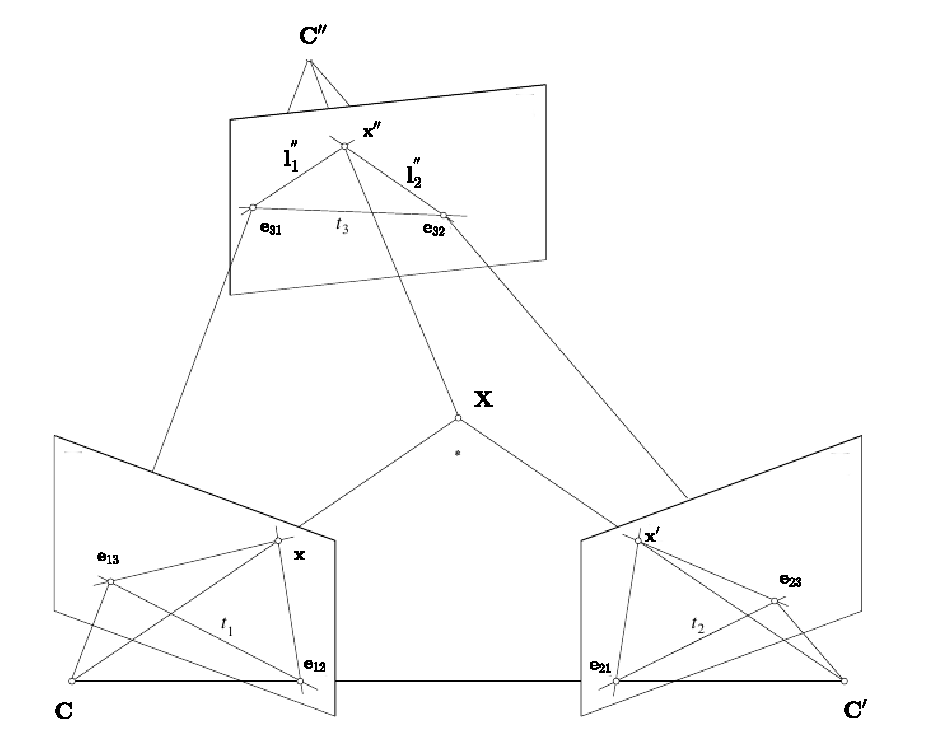
\includegraphics[scale=.8]{trifocal-frente-frente}
\caption{{\it O plano trifocal juntamente com os três planos epipolares. A transferência epipolar falha em alguns casos.}}
\label{fig.trifocal-frente}
\end{figure}

O plano definido pelos pontos $\C, \C' \,\,\text{e}\,\, \X$ forma o plano epipolar para as câmeras 1 e 2. Analogamente, temos o plano epipolar para as câmeras 1 e 3 e para as câmeras 2 e 3. A interseção de cada plano epipolar com os planos das imagens geram as retas epipolares. Por exemplo, a reta  epipolar $\lightrgb''_1$ definida pelos pontos $\e_{31}$ e $\x''$ na terceira imagem, é a reta epipolar com relação ao ponto $\x$ na primeira imagem. Ou seja, $\lightrgb''_1$ é a imagem, na câmera 3, da reta retroprojetada por $\x$ através do centro de projeção $\C_1$ na câmera 1. Essa reta é definida por $\lightrgb''_1=F_{31}\,\x$ ou $\lightrgb''_1=\e_{31}\times\x''$, onde $F_{ij}$ é a matriz fundamental para as câmeras $i$ e $j$ tomando como base a câmera $j$. O plano formado pelos centros de projeção $\C, \C' \,\,\text{e}\,\, \C''$ é chamado {\it plano trifocal} e as interseções desse plano com os planos das imagens geram as {\it retas trifocais} denotadas por ${\bf t}_i$.

\subsubsection{Transferência de pontos usando as matrizes fundamentais}
Supondo que temos o pontos correspondentes $\x\leftrightarrow\x'$ para as câmeras 1 e 2, bem como as matrizes fundamentais para os três planos epipolares da figura \ref{fig.trifocal-frente}, $F_{21}$, $F_{31}$ e $F_{32}$, desejamos determinar as coordenadas do ponto $\x''$ no plano de imagem da câmera 3. Como vimos, os pontos $\x$, $\x'$ e $\x''$ são imagens de um mesmo ponto 3D $\X$, e por isso $\x''$ é um ponto relacionado ao ponto $\x$ e, portanto, $\x''\in\lightrgb''_1$, onde $\lightrgb''_1=F_{31}\x$ é a reta epipolar para as câmeras 1 e 3. Por um argumento similar, constatamos que $\x''$ está relacionado ao ponto $\x'$ e por isso $\x''\in\lightrgb''_2=F_{32}\x'$. Como temos os pontos e as matrizes fundamentais podemos calcular as retas epipolares na terceira imagem. O ponto $\x''$ será calculado como a interseção entre essas duas retas:
\begin{equation}
\begin{array}{rcl}
\x''&=&\lightrgb''_1\times\lightrgb''_2\\
\x''&=&F_{31}\x\times F_{32}\x'.
\end{array}
\end{equation}
Esse metodo é chamado de {\it transferência epipolar} e não podemos determinar $\x''$ nos seguintes casos:
\begin{itemize}
\item acompanhando ainda pela figura \ref{fig.trifocal-frente}, observe que se o ponto 3D $\X$ pertence à reta base definida por $\C$ e $\C''$, então a projeção da primeira câmera será $\x=P\,\X=\e_{13}$, já que $\X$ está alinhado com $\C''$ e $\e_{13}=P\,\C''$. Sendo $\x=\e_{13}$ temos que, pela subseção tal $F_{31}\e_{13}={\bf 0}$, e a reta epipolar $\lightrgb''_1=0$. Geometricamente, não podemos determinar um plano epipolar para as câmeras 1 e 3;
\item analogamente ao caso anterior, se $\X$ pertence a reta base definida por $\C'$ e $\C''$, não podemos definir o plano epipolar para as câmeras 2 e 3;\\

Já que o ponto procurado $\x''$ é calculado como interseção das duas retas epipolares $\lightrgb''_1$ e $\lightrgb''_2$, o procedimento de tranferência falha em mais dois casos quando essas retas são iguais.

\item repare que se os centros de projeção não estão alinhados então os epipolos $\e_{31}$ e $\e_{31}$ são diferentes. As retas epipolares $\lightrgb''_1$ e $\lightrgb''_2$ são iguais se $\e_{31}\in\lightrgb''_2$ e $\e_{32}\in\lightrgb''_1$. Geometricamente, isso significa que o ponto $\X$ está alojado no plano trifocal.

\item se os centros de projeção estão alinhados então os epipolos $\e_{31}$ e $\e_{32}$ são iguais, e daí $\lightrgb''_1=\lightrgb''_2$. Geometricamente, temos infinitos planos passando pela reta definida por $\C$, $\C'$ e $\C''$, e o ponto $\x''$ será indeterminado para qualquer ponto $\X$ no espaço 3D.
\end{itemize}

Todos os casos se resumem ao fato de o ponto $\X$ estar alojado no plano trifocal, pois desse jeito os planos epipolares coincidem com o plano trifocal. Mais ainda, a acurácia do ponto $\x''$ fica bastante prejudicada se $\X$ está próximo do plano trifocal, pois as retas epipolares se tornam menos transversas. 

Mostramos a determinação do ponto $\x''$, mas esse desenvolvimento através da transferência epipolar é análogo para a predição de $\x$ ou $\x'$. Alguns dos casos de degeneração são resolvidos através da introdução de uma nova ferramenta algébrica, o {\it tensor trifocal}.

\subsubsection{O tensor trifocal}
Para a derivação do tensor trifocal usaremos a correspondência entre retas $\lightrgb\leftrightarrow\lightrgb'\leftrightarrow\lightrgb''$ ao longo de três imagens, onde todas essas retas são imagens de uma mesma reta $\bf L$ no espaço 3D, pois esse é o procedimento padrão desenvolvido originalmente por 
\citep{original-trifocal-retas} e reproduzido, por exemplo, por  \citep{Faugeras} e \citep{forsyth}. A abordagem algébrica aqui utilizada pode ser encontrada em \citep{Hartley2004}.

Suponha, portanto, que temos três imagens em 2D $\lightrgb$, $\lightrgb'$ e $\lightrgb''$  de uma reta ${\bf L}$ em 3D, conforme a figura \ref{fig.abord-geo-tri}. Pela subseção \ref{sec.proj.retas}, essas três retas nas imagens retroprojetam planos que, pela própria construção, devem se intersectar em ${\bf L}$. Esta imposição geométrica gera uma restrição algébrica para as três retas correspondentes, já que em geral três planos no espaço não se intersectam numa única reta. Pela subseção tal, através de uma transformação projetiva podemos utilizar o conjunto de matrizes canônicas para as câmeras $P=[I|{\bf 0}]$, $P'=[A|{\bf a}_4]$ e $P''=[B|{\bf b}_4]$, onde $A$ e $B$ são matrizes $3\times3$ e os vetores ${\bf a}_i$ e ${\bf b}_i$ representam a $i$-ésima coluna de suas respectivas matrizes para $i=1,2,3 \,\,\text{e}\,\, 4$.

Observe que tomando $P=[I|{\bf 0}]$ estamos considerando o centro da câmera 1 como a origem de coordenadas do espaço 3D, e assim as coordenadas do centro da câmera 1 é $\C=(0,0,0,1)^\top$. Os epipolos na segunda e terceira imagens em relação à câmera 1 são, respectivamente, dados pela projeção $\e'=P'\C$ e $\e''=P''\C$, e assim temos que $\e'={\bf a}_4$ e $\e''={\bf b}_4$. Como retas retroprojetam planos, esses planos são dados, de acordo com a subseção tal, por
\begin{equation*}
\begin{array}{rcl}
\pi&=&P^\top\lightrgb\\
\pi&=&
\begin{pmatrix}
\lightrgb\\
0
\end{pmatrix}
\end{array},\qquad
\begin{array}{rcl}
\pi'&=&P'^\top\lightrgb'\\
\pi'&=&
\begin{pmatrix}
A^\top\lightrgb'\\
{\bf a}^\top_4\lightrgb'
\end{pmatrix}
\end{array}\quad\text{e}\quad
\begin{array}{rcl}
\pi''&=&P''^\top\lightrgb''\\
\pi''&=&
\begin{pmatrix}
B^\top\lightrgb''\\
{\bf b}^\top_4\lightrgb''
\end{pmatrix}
\end{array}.
\end{equation*}
Como estamos supondo que essas três retas são imagens de uma única reta no espaço, temos que esses três planos devem se intersectar em ${\bf L}$, e essa restrição geométrica pode ser expressa algebricamente pelo fato de que a matriz formada pelos vetores dos planos $M=[\pi \,\,\pi'\,\,\pi'']$ deve ter posto 2. Pois, um ponto $\X\in{\bf L}$ pode ser escrito como combinação linear de outros dois pontos pertencentes a ${\bf L}$ que sejam linearmente independentes, digamos $\X=\lambda_1\X_1+\lambda_2\X_2$, com $\lambda_i$ escalares. Como $\X\in\pi_j$ para $j=1,2,3$ temos que $\pi_j^\top\X=0$ e daí $M^\top\X=0$. Desde que $\X=\lambda_1\X_1+\lambda_2\X_2$, temos que o núcleo de $M^\top$ tem dimensão 2 e portanto $M$ tem posto 2.
\begin{figure}[!htb]
\centering
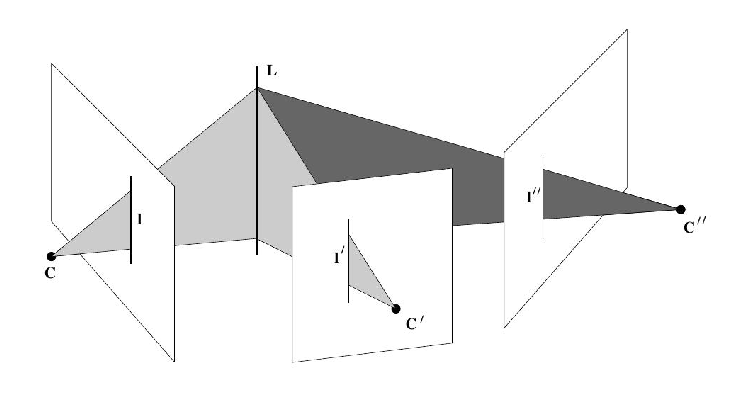
\includegraphics[scale=1]{abord-geo-tri}
\caption{{\it O desenvolvimento algébrico do tensor trifocal realizado a partir das três imagens de uma reta no espaço 3D.}}
\label{fig.abord-geo-tri}
\end{figure}
Considerando $\alpha$, $\beta$ e $k$ escalares, o posto 2 de $M$ pode ser interpretado com uma dependência linear entre suas colunas, e como
\begin{equation*}
M=
\begin{bmatrix}
\lightrgb&A^\top\lightrgb'&B^\top\lightrgb''\\
0&{\bf a}^\top_4\lightrgb'&
{\bf b}^\top_4\lightrgb''
\end{bmatrix}
\end{equation*}
podemos definir o sistema
\begin{equation}\label{eq.sistema-tri}
\begin{pmatrix}
\lightrgb\\
0
\end{pmatrix}
=
\alpha
\begin{pmatrix}
A^\top\lightrgb'\\
{\bf a}^\top_4\lightrgb'
\end{pmatrix}
+\beta
\begin{pmatrix}
B^\top\lightrgb''\\
{\bf b}^\top_4\lightrgb''
\end{pmatrix}.
\end{equation}
Pela quarta equação do sistema \ref{eq.sistema-tri} temos
\begin{equation*}
0=\alpha\,{\bf a}^\top_4\lightrgb'+\beta\,{\bf b}^\top_4\lightrgb''\quad\Leftrightarrow\quad\alpha=k\,{\bf b}^\top_4\lightrgb''\quad\text{e}\quad\beta=-k\,{\bf a}^\top_4\lightrgb'.
\end{equation*}
Substituindo os valores de $\alpha$ e $\beta$ nas três primeiras equações do sistema \ref{eq.sistema-tri} e desconsiderando o fator de escala $k$, temos
\begin{equation*}
\begin{array}{rcl}
\lightrgb&=&\alpha\,A^\top\lightrgb'+\beta\,B^\top\lightrgb''\\
\lightrgb&=&({\bf b}^\top_4\lightrgb'')A^\top\lightrgb'-({\bf a}^\top_4\lightrgb')B^\top\lightrgb''\\
\lightrgb&=&(\lightrgb''^\top{\bf b}_4)A^\top\lightrgb'-(\lightrgb'^\top{\bf a}_4)B^\top\lightrgb''
\end{array}.
\end{equation*}
A $i$-ésima coordenada de $\lightrgb$ pode ser dada por
\begin{equation*}
\begin{array}{rcl}
l_i&=&\lightrgb''^\top({\bf b}_4{\bf a}^\top_i)\lightrgb'-\lightrgb'^\top({\bf a}_4{\bf b}_i^\top)\lightrgb''\\
l_i&=&\lightrgb'^\top({\bf a}_i{\bf b}^\top_4)\lightrgb''-\lightrgb'^\top({\bf a}_4{\bf b}_i^\top)\lightrgb''\\
l_i&=&\lightrgb'^\top({\bf a}_i{\bf b}^\top_4-{\bf a}_4{\bf b}_i^\top)\lightrgb''\\
l_i&=&\lightrgb'^\top \mbox{T}_i\lightrgb'',
\end{array}
\end{equation*}
onde definimos $\mbox{T}_i={\bf a}_i{\bf b}^\top_4-{\bf a}_4{\bf b}_i^\top$. 
O conjunto das três matrizes $\left\{\mbox{T}_1,\mbox{T}_2,\mbox{T}_3\right\}$ é denominado {\it tensor trifocal} e a reta $\lightrgb$ é dada por
\begin{equation}\label{eq.tres-retas}
\lightrgb=
\begin{pmatrix}
\lightrgb'^\top \mbox{T}_1\lightrgb''\\
\lightrgb'^\top \mbox{T}_2\lightrgb''\\
\lightrgb'^\top \mbox{T}_3\lightrgb''
\end{pmatrix}.
\end{equation}

\subsubsection{Homografia induzida por um plano}\label{sec.homo-plano-tri}
Vimos na subseção anterior que podemos determinar o tensor trifocal através da relação entre três retas correspondentes, mas existem mais quatro relações entre retas e pontos  correspondentes envolvendo o tensor trifocal. Para derivarmos essas outras relações e voltarmos ao problema da transferência de pontos, precisamos definir a homografia entre a primeira e terceira imagens induzida por um plano $\bpi'$, retroprojetado por uma reta $\lightrgb'$ na segunda imagem, conforme a figura \ref{fig.transfer-retas}.
\begin{figure}[!htb]
\centering
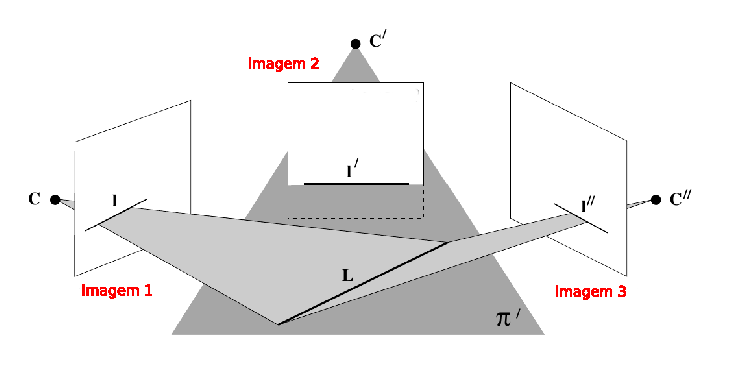
\includegraphics[scale=1]{transfer-retas}
\caption{{\it O plano $\bpi'$ retroprojetado por $\lightrgb'$ induz uma homografia que relaciona $\lightrgb$ com $\lightrgb''$.}}
\label{fig.transfer-retas}
\end{figure}
As homografias entre pontos e retas em dois planos são dadas, respectivamente, por $\x''=H\,\x$ e $\lightrgb''=H^{-\top}\lightrgb$ (subseção \ref{sec.trans-proj-H}). Invertendo $H^{-\top}$ temos que $\lightrgb=H^\top\lightrgb''$. Como temos três retas correspondentes que satizfazem a relação \ref{eq.tres-retas}, podemos comparar essa relação com $\lightrgb=H^\top\lightrgb''$ e deduzir que 
\begin{equation*}
\lightrgb=
\begin{pmatrix}
\lightrgb'^\top \mbox{T}_1\lightrgb''\\
\lightrgb'^\top \mbox{T}_2\lightrgb''\\
\lightrgb'^\top \mbox{T}_3\lightrgb''
\end{pmatrix}=
\begin{pmatrix}
(\mbox{T}_1^\top\lightrgb')^\top\lightrgb''\\
(\mbox{T}_2^\top\lightrgb')^\top\lightrgb''\\
(\mbox{T}_3^\top\lightrgb')^\top\lightrgb''
\end{pmatrix}=
\begin{pmatrix}
{\bf h}_1^\top\lightrgb''\\
{\bf h}_2^\top\lightrgb''\\
{\bf h}_3^\top\lightrgb''
\end{pmatrix}=
\begin{bmatrix}
{\bf h}_1^\top\\
{\bf h}_2^\top\\
{\bf h}_3^\top
\end{bmatrix}\,\lightrgb''=
H^\top\lightrgb'',
\end{equation*}
onde tomamos ${\bf h}_i=\mbox{T}_i^\top\lightrgb'$ e portanto $H=[\mbox{T}_1^\top\lightrgb',\mbox{T}_2^\top\lightrgb',\mbox{T}_3^\top\lightrgb']$.
A homografia deduzida acima representa a transformação de um ponto da primeira imagem para a terceira através de uma reta na segunda imagem, $\x''=H_{13}\x$. Analogamente, podemos deduzir a homografia da primeira imagem para a segunda através de uma reta na terceira imagem, $\x'=H_{12}\x$.

\subsubsection{Relações de incidência entre pontos e retas}
Uma das relações de incidência já foi deduzida anteriormente, chamada reta-reta-reta, e agora vamos deduzir mais quatro relações. Supondo ainda $\lightrgb$, $\lightrgb'$ e $\lightrgb''$ três imagens de uma reta ${\bf L}$, sabemos que um ponto $\x$ pertence à uma reta $\lightrgb$ na câmera 1 se $\x^\top\lightrgb=0$, onde a multiplicação matricial pode ser escrita sob a notação de somatório como $\sum_{i=1}^{3}x^il_i$. A equação \ref{eq.tres-retas} pode ser dada como $\lightrgb'^\top \mbox{T}_i\lightrgb''
=l_i$ para $i=1,2,3$, e substituindo o somatório temos que
\begin{equation*}
\begin{array}{rcl}
\lightrgb'^\top \mbox{T}_i\lightrgb''
&=&l_i\\
\sum_{i=1}^3 x^i\lightrgb'^\top \mbox{T}_i\lightrgb''&=&\sum_{i=1}^3 x^il_i\\
\lightrgb'^\top(\sum_{i=1}^3 x^i\mbox{T}_i)\lightrgb''&=&0.
\end{array}
\end{equation*}
Desta forma, temos uma relação de incidência chamada ponto-reta-reta, para um ponto $\x$ na primeira imagem e as retas $\lightrgb'$ e $\lightrgb''$ na segunda e terceira imagens respectivamente. 

Pela subseção \ref{sec.proj.retas} sabemos da existência de um ponto $\X\in{\bf L}$ que projeta $\x\in\lightrgb$ na primeira imagem e projeta a outros dois pontos $\x'\in\lightrgb'$ e $\x''\in\lightrgb''$, ou seja, temos a correspondência $\x\leftrightarrow\x'\leftrightarrow\x''$. Assim, podemos deduzir as relações para 
pontos na segunda e terceira imagens utilizando a homografia induzida por plano, e vamos tratar do caso ponto-reta-ponto. Usando o resultado da subseção \ref{sec.homo-plano-tri} temos que 
\begin{equation*}
\begin{array}{rcl}
\x''&=&H_{13}\x\\
&=&[\mbox{T}_1^\top\lightrgb',\mbox{T}_2^\top\lightrgb',\mbox{T}_3^\top\lightrgb']\x\\
&=&
\begin{pmatrix}
x_1\mbox{T}_1^\top\lightrgb'+x_2\mbox{T}_2^\top\lightrgb'+x_3\mbox{T}_3^\top\lightrgb'
\end{pmatrix}\\
&=&(\sum_{i=1}^3 x^i\mbox{T}_i^\top)\,\lightrgb'
\end{array}
\end{equation*}
Como estamos expressando os vetores em coordenadas homogêneas, essas equações são invariáveis para a aplicação de um fator de escala. De qualquer maneira, podemos eliminar o problema das diferenças de escala aplicando a transposição seguida do produto vetorial em ambos os lados da equação.
\begin{equation}\label{eq.ponto-reta-ponto}
\begin{array}{rcl}
\x''&=&(\sum_{i=1}^3 x^i\mbox{T}_i^\top)\,\lightrgb'\\
\x''^\top&=&\lightrgb'^\top(\sum_{i=1}^3 x^i\mbox{T}_i)\\
\x''^\top[\x'']_\times&=&\lightrgb'^\top(\sum_{i=1}^3 x^i\mbox{T}_i)[\x'']_\times\\
{\bf 0}^\top&=&\lightrgb'^\top(\sum_{i=1}^3 x^i\mbox{T}_i)[\x'']_\times
\end{array}
\end{equation}
O quarto caso, ponto-ponto-reta, é análogo ao apresentado aqui substituindo $\x''$ por $\x'$, e usando a homografia induzida pelo plano retroprojetado por $\lightrgb''$, $\x'=H_{12}\x$.

Por último, temos a relação de incidência para três pontos. 
Observe que a reta $\lightrgb'$ pode ser definida como $\lightrgb'=\x'\times \y'=[\x']_\times \y'$, já que $\x'\in\lightrgb'$ e $\y'$ é um ponto qualquer no plano da segunda imagem. Substituindo $\lightrgb'$, a relação \ref{eq.ponto-reta-ponto} se torna 
\begin{equation*}
\y'^\top[\x']_\times(\sum_{i=1}^3 x^i\mbox{T}_i)[\x'']_\times={\bf 0}^\top,
\end{equation*}
mas observe que tal relação é válida para qualquer reta $\lightrgb'$ que seja imagem de ${\bf L}$, e portanto não depende da escolha do ponto $\y'$ que pode ser descartado. A relação ponto-ponto-ponto é
\begin{equation*}
[\x']_\times(\sum_{i=1}^3 x^i\mbox{T}_i)[\x'']_\times=0_{3\times3}.
\end{equation*}
Cabe resaltar que apenas satisfazer qualquer das relações de incidência não garante a incidência no espaço 3D, ou seja, os resultados obtidos podem não ter consistência com a geometria trifocal de abordagem do problema.




























\subsection{Pesquisa Anterior para Determinação de Câmera usando três Imagens}


\subsubsection{Abordagem de Schimd e Zisserman}

Este artigo lida com o problema de encontrar correpondências entre seguimentos de curvas quando temos diponíveis duas ou três imagens de câmeras deconhecidas. A matriz fundamental e o tensor trifocal são facilmente computados através de pontos de interesse mais o uso do RANSAC, mas os parâmetros intrínsecos não precisam necessariamente ser conhecidos. A abordagem clássica é descartar esses pontos de interesse e usar a geometria da câmera em estágios subsequentes de associação estéreo, para eliminar a ambiguidade entre pontos correspondentes ao longo da linha epipolar. Com duas imagens, o método padrão é usar a restrição epipolar para computar pontos correspondentes, o qual limita os canditados a estarem numa região estreita, e o uso de correleção cruzada normalizada, obtida a partir de fotometria, para restringir mais ainda nossas escolhas dos pontos. 

No artigo são analisados dois casos, binocular e trinocular, para responder a uma questão principal: existe alguma restrição adicional quando não utilizamos pontos mais sim pontos-tangentes ou geometria de curvas em geral disponíveis?\\

\noindent {\bf O Caso Binocular}

A busca por correspondências usando correlação fotométrica pode ser significantemente reduzida usando geometria de curvas (sem a utilização de contornos oclusos) numa pequena vizinhança. Considere uma aproximação de primeira ordem (planar) para a superfície de um objeto no qual aloja-se uma curva 3D. A correspondência entre as projeções desse plano em duas imagens são descritas por uma homografia de 8 parâmetros livres. É sabido que a matriz fundamental, que contém informações da geometria epipolar, fornece 5 restrições, o que reduz para 3 os graus de liberdade da homografia. Assim, o fato de que um ponto está associado a um outro ponto na reta epipolar já está sendo considerado nos cálculos. Dados alguns pontos correspondentes num fragmento de curva ao longo da linha epipolar, cada par de correspondência fornece duas restrições nas variáveis desconhecidas: como as curvas devem ser mapeadas umas nas outras, (i) a posição ao longo da linha epipolar define uma variável, já que o plano 3D é forçado a passar pelo ponto 3D reconstruído a partir dessa informação (a menos de uma homografia 3D). Assim, resta uma família de um parâmetro que pode ser otimizado usando o grau da correlação fotométrica. Dentre a família de um parâmetro de solução restante, os autores propuseram que, no lugar de otimizar através de correlação fotométrica, podemos apenas escolher o plano que coincide com o plano osculante da curva, o qual pode ser determinado usando a curvatura dos pontos correspondentes. Isto é apenas uma heurística, um método construtivo, onde não há garantia de que se trata da tangente à superfície, mesmo se a curva é plana. Contudo, empiricamente os autores expuseram que essa solução é boa o suficiente para criar uma fila ordenada das associações mesmo considerando os casos acima.

A questão de como conseguir um plano osculante (e a homografia associada a ele) foi a motivação para chegar a um resultado de interesse geral. Sabemos, através da posição e curvatura das extremidades correspondentes em duas imagens, que é possível estimar, unicamente, o plano osculante a uma curva se a calibração da imagem é completamente conhecida. Se apenas a matriz fundamental é conhecida, o plano osculante pode ser encontrado a menos da ambiguidade projetiva somente, mas a homografia associada a ele pode ser completamente determinada, o que é estudado nesse artigo.

\noindent {\bf O Caso Trinocular}

Os autores também propuseram um método para transferir a curvatura de duas imagens para uma terceira, dado um tensor trifocal (a calibração completa não é necessária). A interpretação da fórmula dada é usar o plano reconstruído a partir de duas imagens (conhecido a menos de uma ambiguidade projetiva 3D), e usá-lo para conseguir uma homografia relacionando as duas primeiras imagens com a terceira (sendo esta homografia independente dos parâmetros intrínsecos). Esta homografia define, então, a correspondência de pontos de quaisquer das duas primeiras imagens para a terceira. Faugeras e Robert foram os primeiros a proporem a transferência de curvatura a partir de duas imagens não calibradas para uma terceira, mas eles usaram par de matrizes fundamentais. O enriquecimento adicionado ao método de Faugeras proposto por Chimd e Zisserman é numericamente estável e imune a erros na interseção de linhas epipolares, que podem ser colineares ou aproximadamente colineares. O tensor trifocal manipula esses casos sem qualquer imprecisão.\\

\noindent {\bf Passo para um Sistema Prático} 

\begin{itemize}
\item Começar com a detecção de extremidades relacionadas em duas ou três imagens, e tentar associar fragmentos de curvas por inteiros.
\item Num primeiro estágio, considere apenas curvas alojadas no raio das linhas epipolares de cada uma das outras curvas, e têm tangências epipolares consistentes.
\item Num segundo estágio, tente encontrar fragmentos correspondentes de supostas curvas correspondentes através da integração do custo de extremidade-a-extremidade com possibilidade de associar fragmentos.
\item Usando apenas a geometria diferencial de curvas ganha-se restrições através de supostas extremidades associadas na terceira imagem. Isto funciona mesmo quando os parâmetros intrínsecos são desconhecidos, mas a ambiguidade permanece.
\item Restrições adicionais podem ser encontradas usando as aparências.
\item Para cada suposta associação, encontre um grupo de correlações no espaço gerado por um parâmetro se as curvaturas das associações são poucas (somente tangentes são utilizadas), ou não use buscas (planos osculantes) se as curvaturas acima são limites.
\item Um esquema das melhores escolhas dentre todas direciona para as associações finais.
\end{itemize}



